\begin{figure*}
	\newcommand*{\siftwidth}{.5\linewidth}
	\newcommand*{\length}{sqrt((2.*x^2+2.*y^2)^2 + (8.*x^2*y^2)^2 )}
	\pgfplotsset{ % Define a common style, so we don't repeat ourselves
		dominantorientationaxis/.style={
				enlargelimits = false ,
				view={0}{90},
				xmin=0, xmax=1, ymin=0, ymax=1,
				ytick distance=1/16,
				xtick distance=1/16,
				axis equal image, grid=both,
				minor grid style={black},
				major grid style={black},
				axis equal image,
				samples=16
			},
		dominantorientationvectors/.style={
				domain=1/32:31/32,
				black,
				quiver={
						u={(2.*x^2+2.*y^2)/(2*\length)},
						v={8.*x^2*y^2/(2*\length)},
						scale arrows=0.2},
				-latex
			}
	}
	\pgfplotsset{ticks=none}
	\begin{subfigure}{\siftwidth}
		\centering
		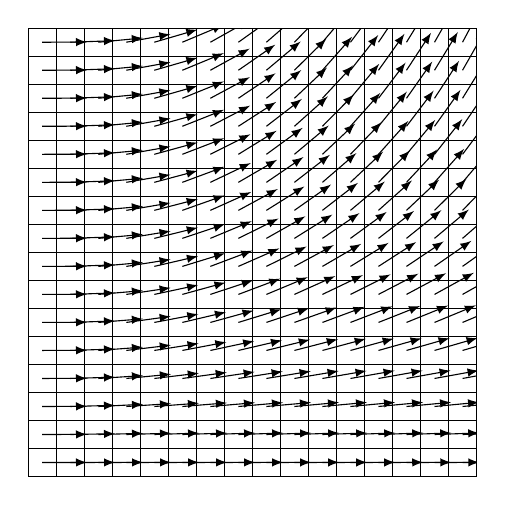
\begin{tikzpicture}[]
			\begin{axis}[dominantorientationaxis]
				\addplot3[dominantorientationvectors] {0};
			\end{axis}
		\end{tikzpicture}
		\caption{First subfigure} \label{fig:1a}
	\end{subfigure}
	\tikzset{
		pics/greensquare/.style args={#1/#2/#3}{
				code = {
						\draw[green] (#1,#2) rectangle (#1+#3, #2+#3);
					}
			},
		gradbins/.pic={
				\foreach \x in {0,1,2,3} {
						\pgfmathtruncatemacro{\angle}{45+\x*90}
						\pic[rotate around={\angle:(0.5,0.5)}] {greensquare=.5/.5/.353};
					}
			},
		subgradbin/.pic={
				\foreach \i in {0.0, 1.0} {
						\pgfmathsetmacro{\x}{0.5+\i*2*.08825};
						\foreach \j in {0.0, 1.0} {
								\pgfmathsetmacro{\y}{0.5+\j*2*.08825};
								\pic[] {greensquare=\x/\y/2*.08825};
							}
					}
			},
		subgradbins/.pic={
				\foreach \x in {0,1,2,3} {
						\pgfmathtruncatemacro{\angle}{45+\x*90}
						\pic[rotate around={\angle:(0.5,0.5)}] {subgradbin};
					}
			},
		edgehistogram/.pic={
				\begin{axis}[area style, width=2.5cm,height=2.5cm, hide axis]
					\addplot+[ybar interval] plot coordinates {
							(-0.50, 2) (0.5, 4) (1.5, 5) (2.5, 3) (3.5, 2) (4.5, 2) (5.5, 0)
						};
					\path
					\foreach[count=\i from 0] \v in {2, 4, 5, 3, 2, 2} {
							(\i, \v) node[below] {\tiny\v}
						};
				\end{axis}
			}
	}
	\begin{subfigure}{\siftwidth}
		\centering
		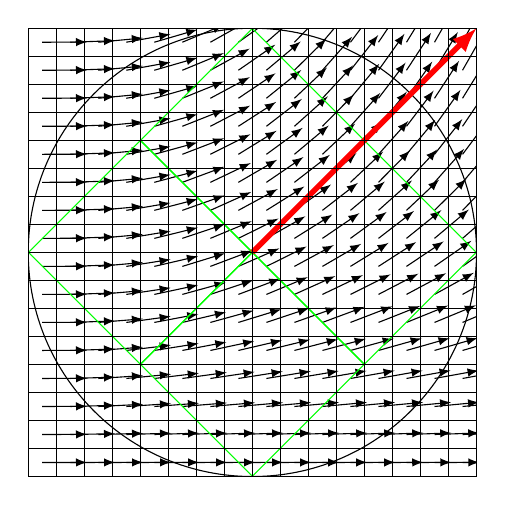
\begin{tikzpicture}[]
			\begin{axis}[dominantorientationaxis]
				\addplot3[dominantorientationvectors] {0};
				\draw (0.5, 0.5) circle [blue, radius=.5];
				\pic[] {gradbins};
				\draw[line width=2pt,red,-latex](.5,.5)--(1,1);
			\end{axis}
		\end{tikzpicture}
		\caption{First subfigure} \label{fig:1b}
	\end{subfigure}
	\vskip\baselineskip

	\begin{subfigure}{\siftwidth}
		\centering
		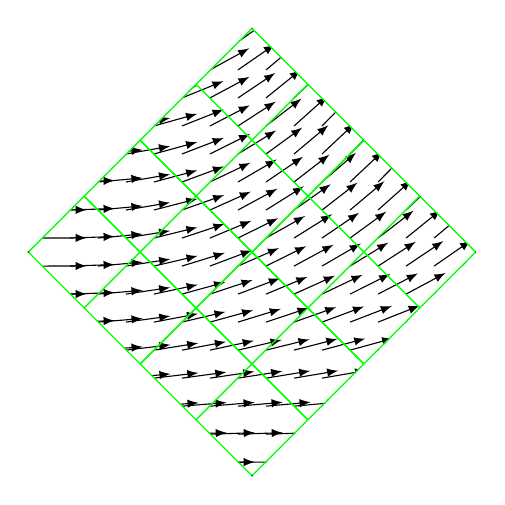
\begin{tikzpicture}[rotate=-45,transform shape]
			\clip[](2.04,2) rectangle (6.07,6.03);
			\begin{axis}[dominantorientationaxis, rotate around={45:(.5,.5)}, grid=none]
				\addplot3[dominantorientationvectors] {0};
				\pic[] {gradbins};
				\pic[] {subgradbins};
			\end{axis}
		\end{tikzpicture}
		\caption{First subfigure} \label{fig:1b}
	\end{subfigure}
	\begin{subfigure}{\siftwidth}
		\centering
		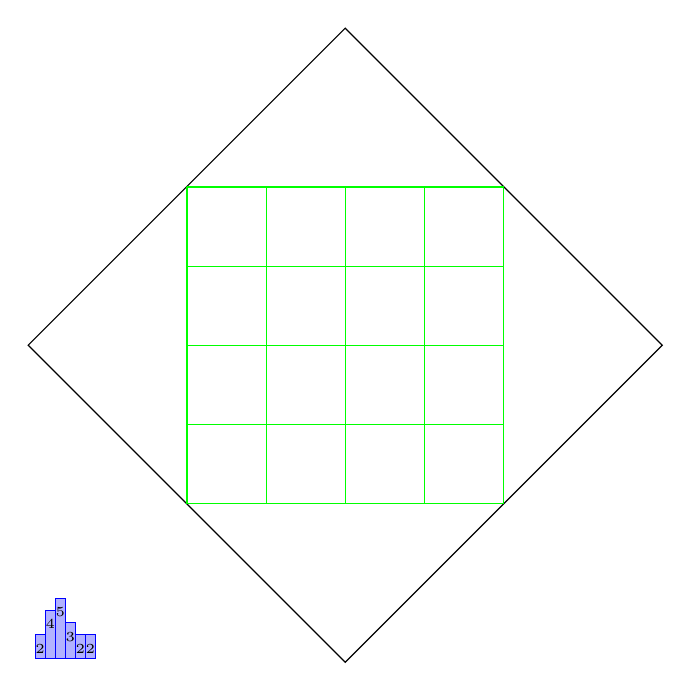
\begin{tikzpicture}[rotate=0,transform shape]
%			\clip[](2.04,2) rectangle (6.07,6.03);
			\begin{axis}[dominantorientationaxis, rotate around={-45:(.5,.5)}, grid=none]
				\pic[] {gradbins};
				\pic[] {subgradbins};
%%				\addplot3[dominantorientationvectors] {0};
			\end{axis}
			\pic {edgehistogram};
		\end{tikzpicture}
		\caption{First subfigure} \label{fig:1b}
	\end{subfigure}
	%	\caption{A figure that contains three subfigures} \label{fig:1}
\end{figure*}

